\section{What is network machine learning?}
\label{sec:ch1:whatis}

If you are reading this book, you probably have some idea what the term ``machine learning'' means. According to wikipedia \cite{wikiML}, machine learning is a field of inquiry devoted to understanding and building methods that {learn}; that is, methods that leverage data to improve performance on some set of tasks.

For instance, if you have an image and you are a photo editor working in pattern recognition, you might want to learn how you can automatically segment a person so that you can blur the background, (see Figure \ref{fig:ch1:ml-ex}. ) If you are doing natural language processing, you might want to learn how identify the unique instruments in the song on an audio track. If you are a scientist, you might want to learn how a lobster's size correlates with its age so that you can predict lobsters' average age.  What unites these examples is that in all of them you are using data,  to learn something so that you can accomplish some task. Machine learning has grown enormously over the past few decades, and the use-cases of machine learning are rapidly coming to pervade modern life.

\begin{figure}[h]
    \centering
    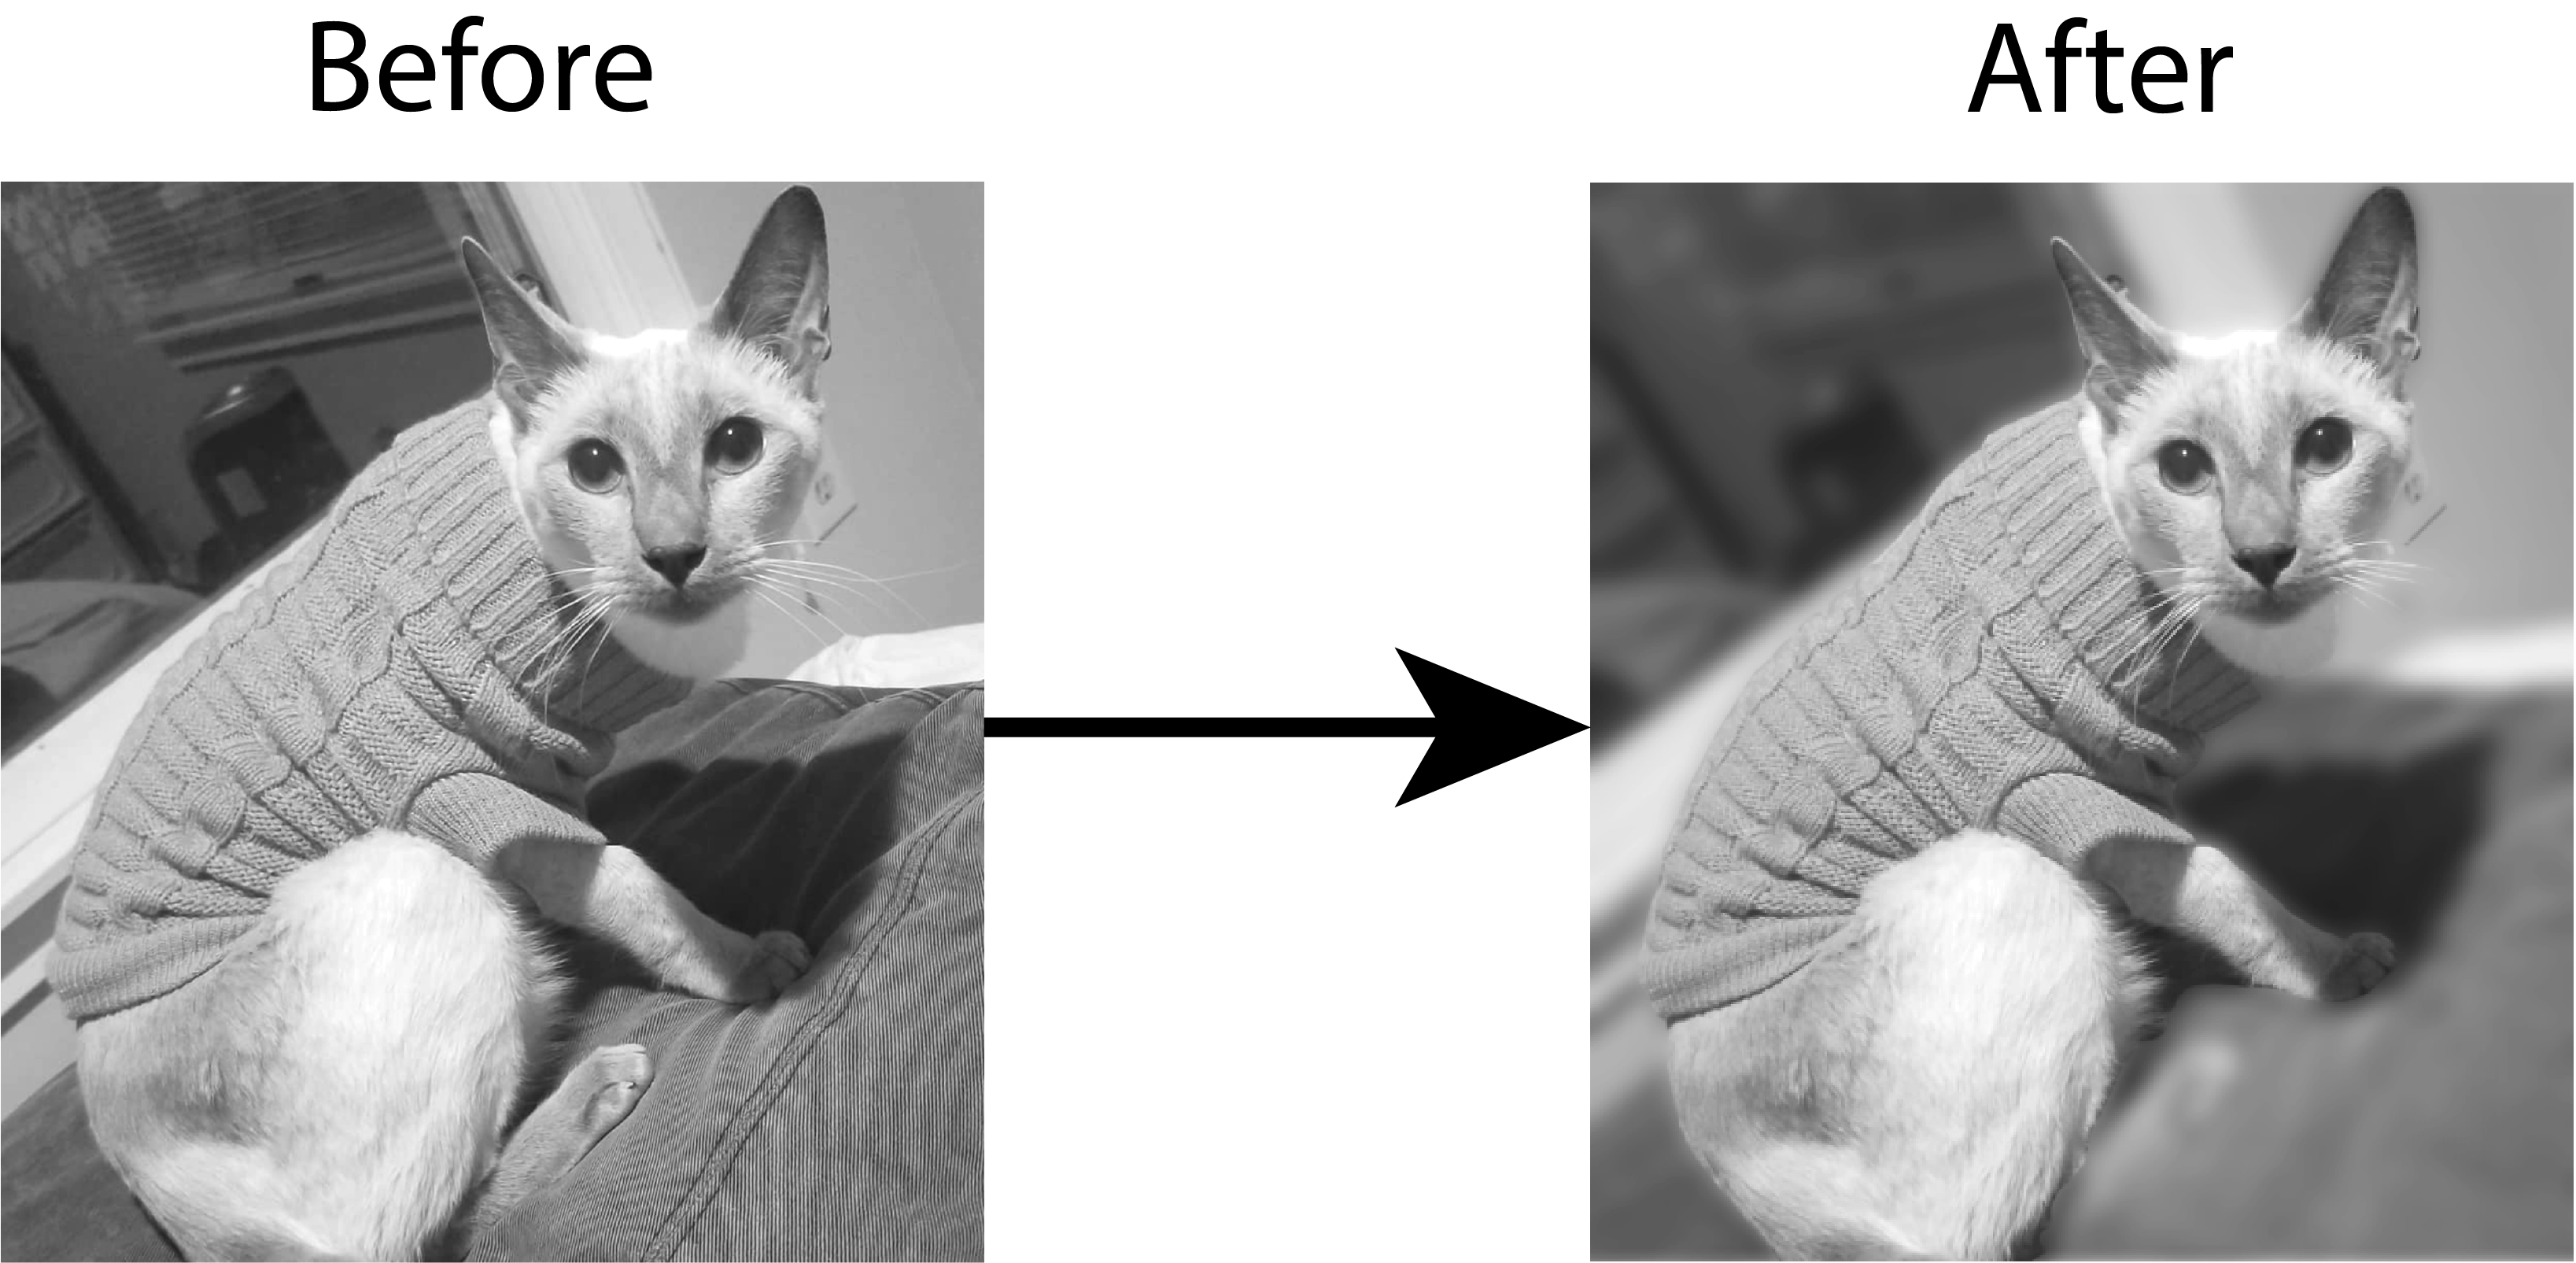
\includegraphics[width=\linewidth]{foundations/ch1/Images/cboy.png}
    \caption[Machine learning task]{Learning how to segment an image to blur the background. A machine learning system is trained using numerous images with the foreground segmented out. This trained system is then used to segment out the foreground on new images, and then the background is blurred.}
    \label{fig:ch1:ml-ex}
\end{figure}


\subsection{Traditional machine learning leverages tabular data structures}

In traditional machine learning, data follows what is called a \textit{tabular} format. This means that the data are arranged in a table or an array, where each row represents a single observation. We recommend you check out the Pandas tutorial on tabular data \cite{pandastut}. 

Conveniently, a lot of modern developments in machine learning apply directly to tabular data. This means that, with some amount of effort, one can take techniques developed in one domain of machine learning, and readily modify or apply them to problems in another domain of machine learning, without needing to {reinvent the wheel}. By this we mean that you can focus your effort on your problem, and borrow techniques developed for related problems, without having to start from scratch every time. For example, if you had a tabular dataset where each row represented a lobster with two columns representing the length and sex of the lobster, you might try to learn how these columns can be used to predict the lobster's claw size. You could do this using an extremely general approach, by simply producing a line of best fit for the claw size depending on which biological sex a lobster is. 

In Figure \ref{fig:ch1:tabular-dat}, we look at how tabular data fits into a machine learning system. This example comprises a basic classification task, in which each observation is either blue or orange. Some of the data (the {training set}, circles) is used to train a machine learning algorithm ({learning}, the transparent blue and orange voronoi cells), and the remainder of the data is used to test the trained algorithm on new data ({evaluating} on the squares using the voronoi cells learned). The trained model can then be further refined ({updated}), or deployed for your intended use-case.

\begin{figure}[h]
    \centering
    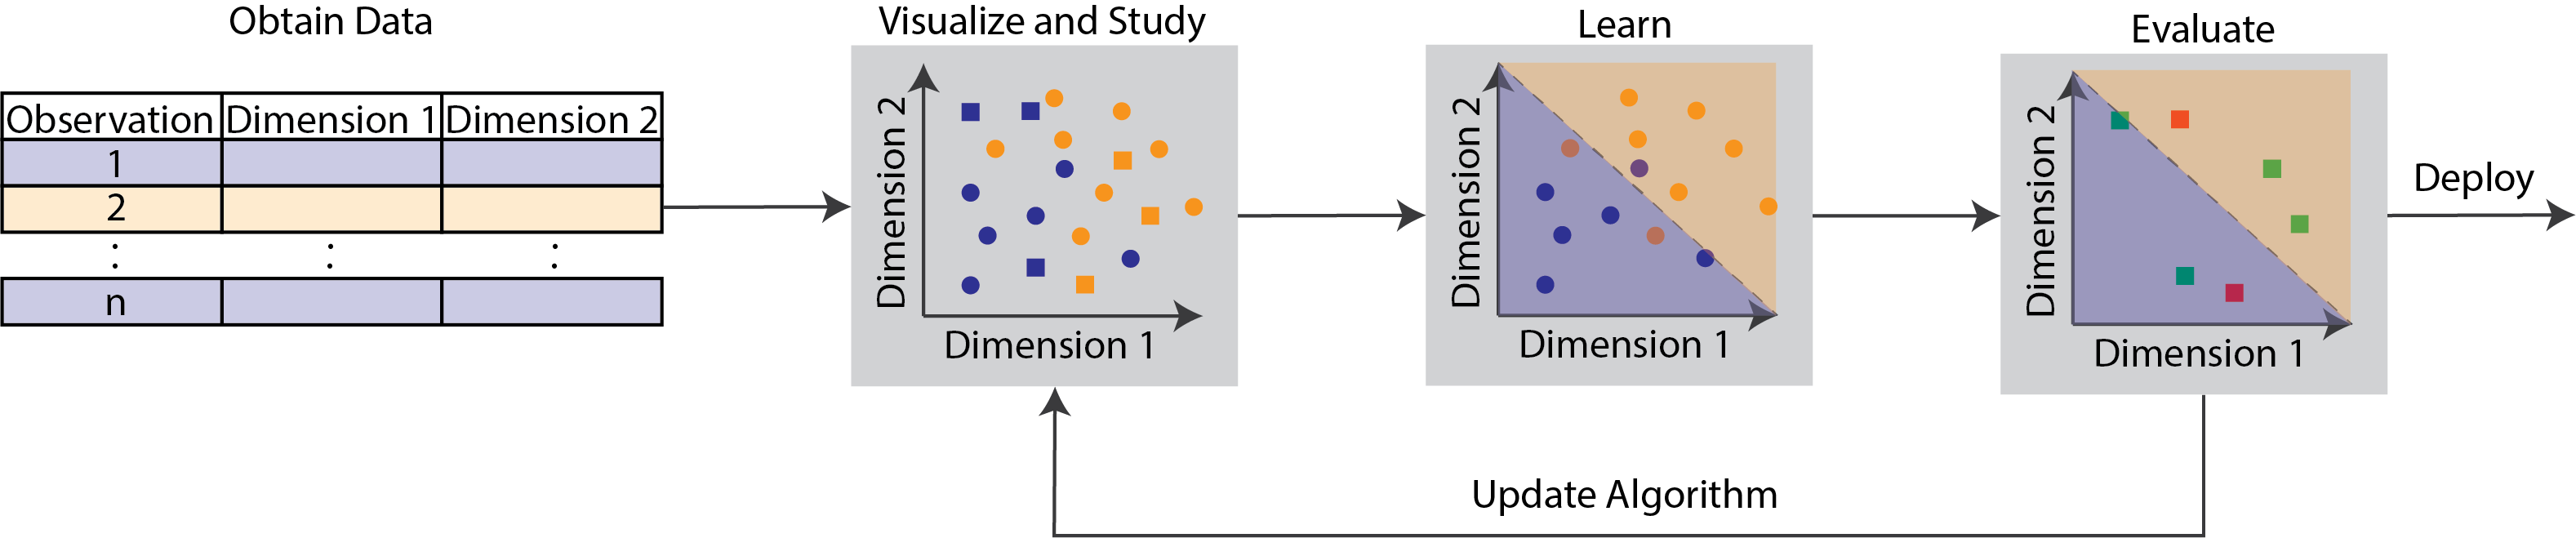
\includegraphics[width=\linewidth]{foundations/ch1/Images/ml_ex.png}
    \caption[Machine learning system]{Machine learning systems start by obtaining inputs as tabular data, where the rows are observations and the columns are features, i.e.  \textit{dimensions} of each observation.}
    \label{fig:ch1:tabular-dat}
\end{figure}

\subsection{What is a network?}

So, what does this have to do with networks? As it turns out, in the 21st century, networks are all around us. When most people think of a ``network'', they often have some vague image in their head of the internet, or of cell phone towers transmitting data, or of some other technical system. But networks have a specific definition in the world of machine learning and data science. The most direct example can easily be explained through the recent rise in social media over the last decade. In a network, your data follows a prescribed pattern: a group of items (say, people on the social network) are interconnected to one another through clearly defined relationships (say which people are friends with one another in the network). 

In other places, you might hear networks referred to as ``graphs'', and the field studying them as ``graph theory''. We try to avoid this terminology in this book, since it's easy to confuse a graph and a plot with an $x$/$y$ coordinate axis. We'll stick to the term ``network'' throughout this book when possible. There might be times when we choose to use the word ``graph'', since the name of some algorithm or tool we're showing you uses it, but just remember that they mean the same thing.

\begin{figure}[h]
    \centering
    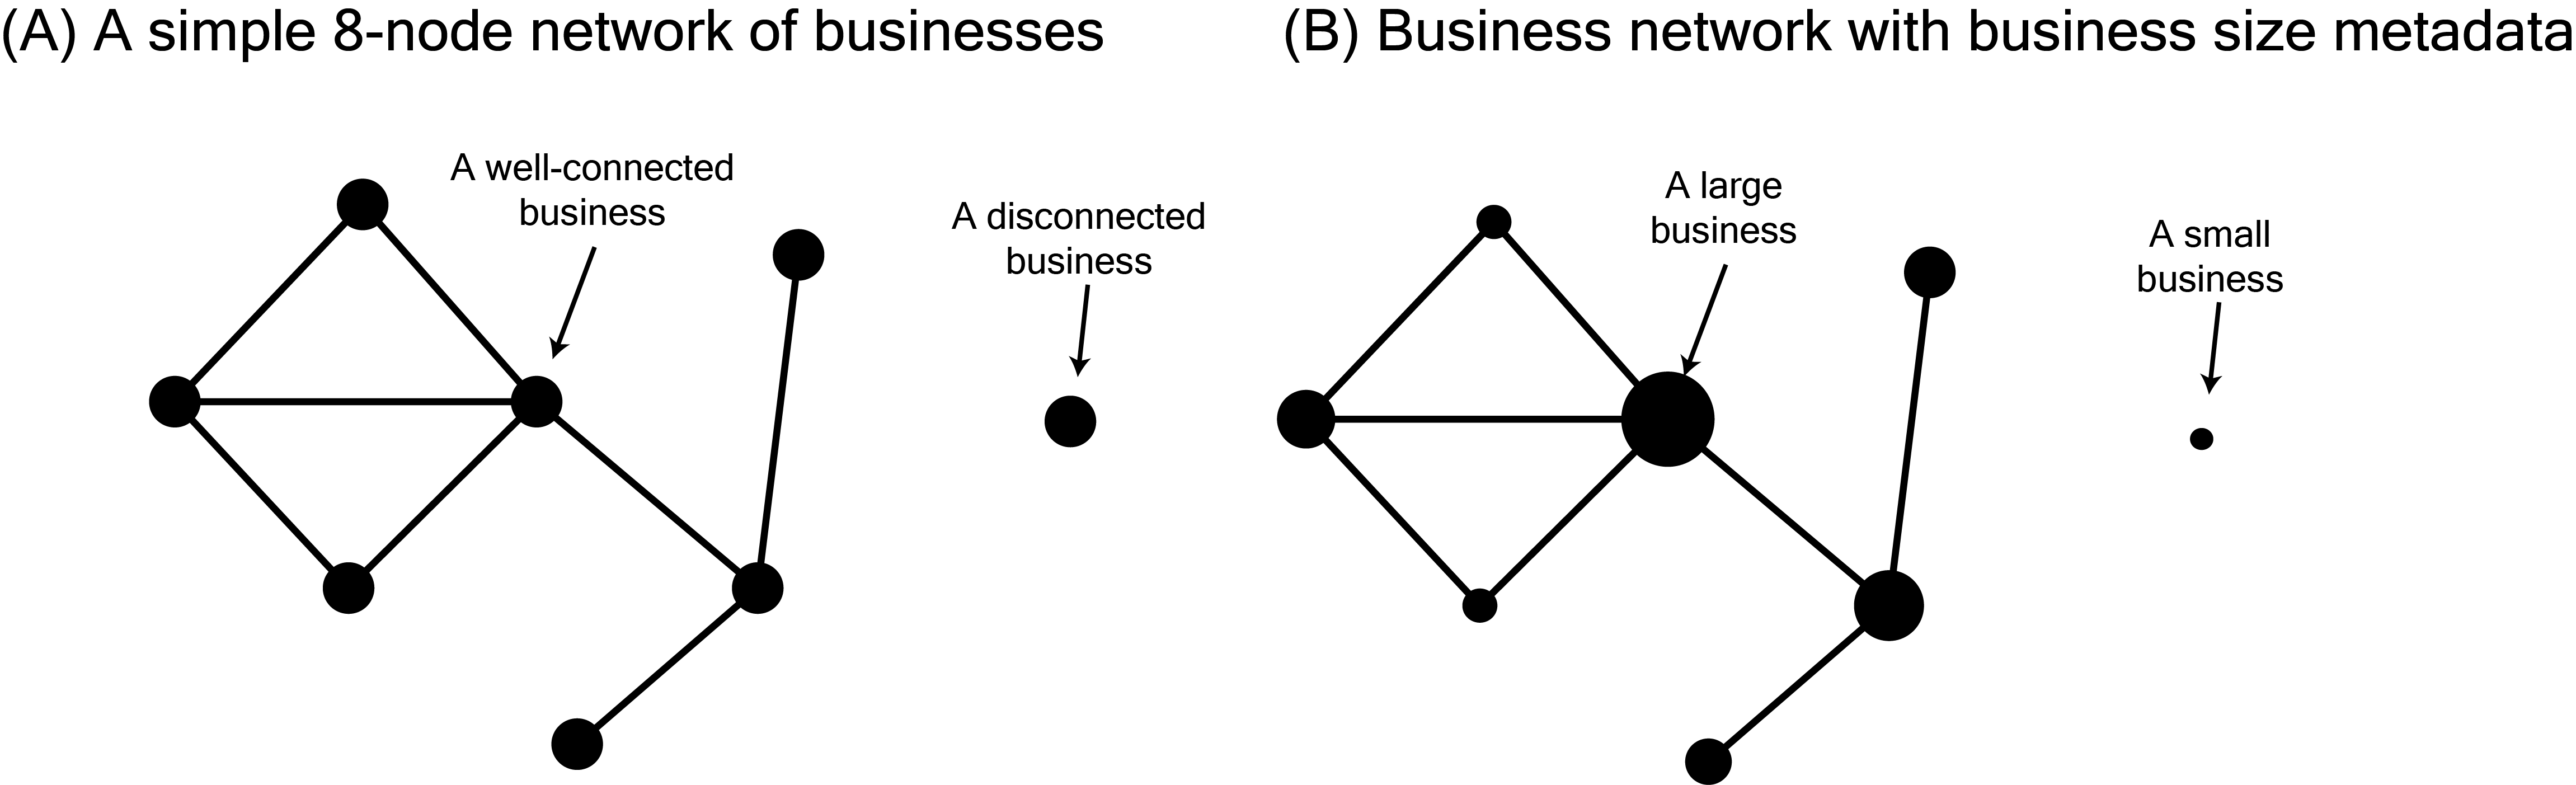
\includegraphics[width=\linewidth]{foundations/ch1/Images/simp_net.png}
    \caption[Simple network example]{\textbf{(A)} indicates a simple network, where nodes are businesses, and edges exist if a given pair of businesses transact with one another. \textbf{(B)} indicates the same simple network, but each node also has a piece of information attached to it, the number of employees (indicated by the node size).}
    \label{fig:ch1:simplenet}
\end{figure}

Let's get more specific about what we mean. Each object in your network is called a \textit{node}, or a vertex (for consistency we'll stick to "node" in this book). A connection between two nodes is called an \textit{edge}. Below you can see a visualization of a simple network with 8 nodes. As you can see, some nodes are well-connected with other nodes -- for example, the node in the center, has edges to five other nodes -- and you can also have nodes which aren't connected to anything, like the lonely extra node without any edges. This is illustrated in Figure \ref{fig:ch1:simplenet}(A).

Networks might also contain extra information. Each node might have a set of features attached to it: extra information that comes in the form of a table. Say the network we just made represents business transactions. Assume that there are eight companies, one corresponding to each node, and there is an edge if one company has sold something to another.

Then, we might also have information about the company size. If the company is larger, you might assume that it'll tend to have had more business transactions with the other companies. The network, in this case, includes the company size information. This is illustrated in Figure \ref{fig:ch1:simplenet}(B).

\subsection{Why do we study networks?}
\label{sec:ch1:howstudy}

If you think about it, you can see networks everywhere. The objects could be people, and the edges could be friendships. Or the objects could be computers, and the relationship could be the information they send to each other. if you're working in air traffic control, you'd have flight networks where the edges are flights from City A to City B; or if you're an epidemiologist studying disease, you could create an infection network. Neuroscientists explore brain networks, consisting of neurons and their relationships with each other, and computer scientists often use neural networks, which have become pillars of machine learning.

Networks can even be used to visualize ideas: in a Bayesian network, nodes represent a set of variables and the edges represent their conditional dependencies. In a correlation network, nodes represent variables, and the edges represent the correlation between those variables. You can have ecological networks, electrical networks, gene networks, or you could visualize your team's workflow with a network.

Even the way we think can be thought of as a network. Visualize a concept or object in your head. Maybe you could think about the food you had for breakfast this morning, or the city you live in. Now, think about the connections between those concepts and others. Maybe you had eggs and toast for breakfast. Eggs and toast are connected with a multitude of other concepts in your head: forks and silverware, kitchens, hunger, protein, carbohydrates, your morning routine, chickens, wheat, other breakfast foods, and innumerable other things. What you're doing right now is exploring a small part of the massive semantic network that exists in your head.

Network machine learning is a relatively new field. The vast majority of it has been invented (or discovered) after the year 2000, and many fundamental proofs have only been published recently. 

For the business-minded readers out there, this is an incredible time to learn about networks. Graph neural networks (GNNs) are becoming increasingly popular as deep learning and neural networks proliferate. This book provides the basic foundational concepts and intuition required to understand how, when, and why GNNs, or any other network machine learning tool, work.

Real-life applications also follow a general trend. It begins with academics spending a lot of time, usually 10-20 years, publishing proof-of-concept papers, discussing possible approaches to solve problems, and developing fundamental tools (usually informally, with somewhat messy code that exists in jupyter notebooks). Then, as the field of research starts maturing, companies and industry people start noticing these new academic tools. They find ways to apply them to make their product or service better, and they develop easy-to-use packages like \texttt{scikit-learn} to make these academic tools mainstream. Network machine learning is at a tipping point right now: its academic foundations have been built up over the past 10-20 years, and the tools for building and working with networks are now starting to move from academia to industry. Congratulations: you could get in early for a wave of application-focused network machine learning tools!


\subsubsection{Why do we need special machine learning approaches for networks?}

As you will learn throughout this book, the problem you run into is that networks mostly exist not in their most naive form, tabular data, but instead in network-valued data. This means, unfortunately, that all those techniques that were developed over decades for tabular data cannot, natively, be used for network-valued data. However, as we will see, we can take various approaches to {adapt} networks to a more traditional format, including tabular structures using network representations. Once we adapt these networks  to more traditional structures, we can then apply techniques from other domains of machine learning to learn about our networks. In Figure \ref{fig:ch1:nml-high-level}, we see how network machine learning functions at a high level. Loosely, \textit{network machine learning} is machine learning for network-valued data (data which is a {network}, not a {tabular structure}). 

\begin{figure}
    \centering
    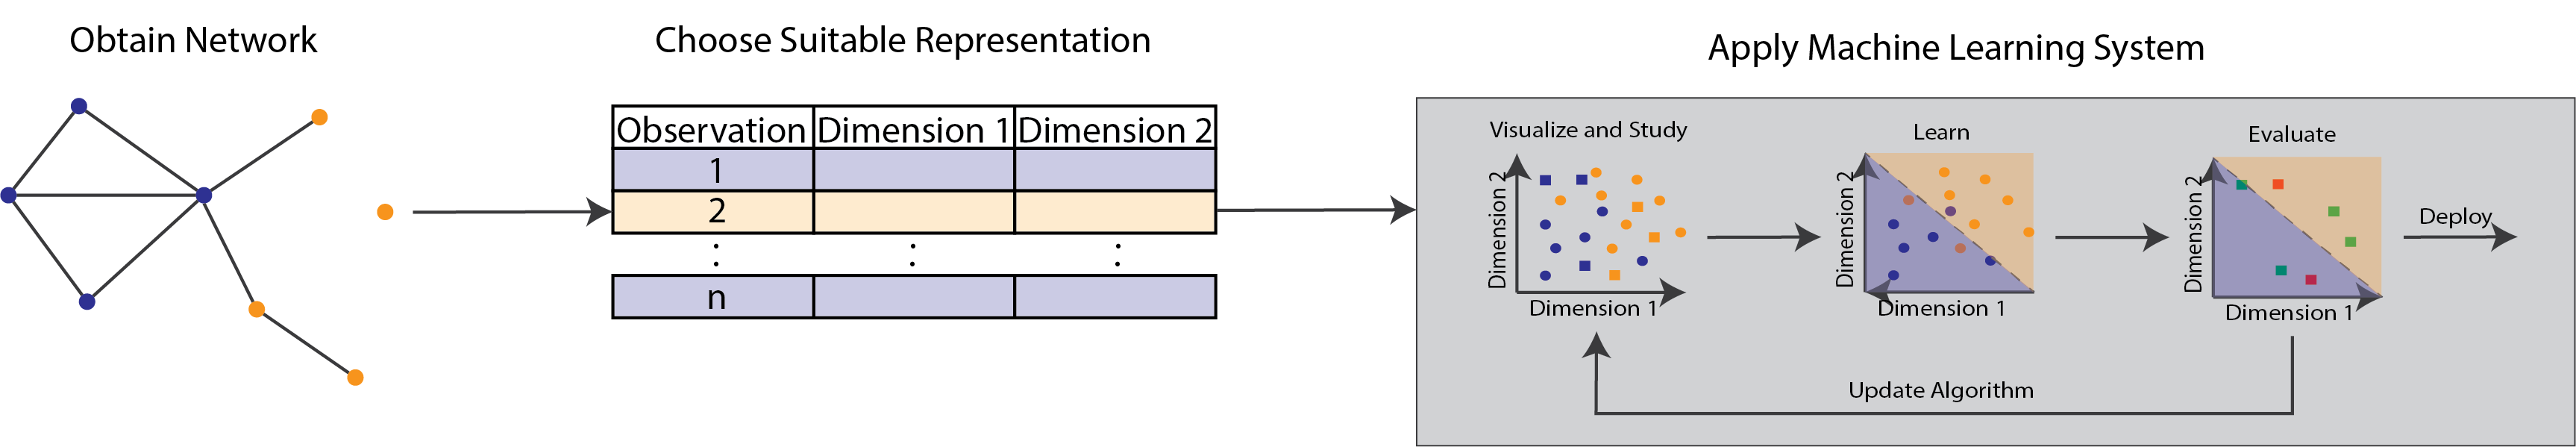
\includegraphics[width=\linewidth]{foundations/ch1/Images/nml-high-level.png}
    \caption[Network machine learning]{In network machine learning, we start by obtaining a network. The first step in network machine learning is to select a suitable representation for the network, which depends on the type of questions you are asking. Using this representation, you apply a machine learning system which is suited appropriately for the type of task that you have. As the set of questions one might have about network data may differ from a typical tabular dataset, the manner in which these techniques are applied may need to be tuned for the question of interest.}
    \label{fig:ch1:nml-high-level}
\end{figure}



Let's get started!

\newpage